% 
% Originally from Jeff Philips, University of Utah
%
\documentclass[11pt]{article}

\usepackage{euscript}
\usepackage{amsmath}
\usepackage{amsthm}
\usepackage{amssymb}
\usepackage{epsfig}
\usepackage{xspace}
\usepackage{color}
\usepackage{url}
\usepackage{graphicx}
\usepackage{subcaption}
%\usepackage{floatrow}
%\usepackage{wrapfig}



%%%%%%%  For drawing trees  %%%%%%%%%
%\usepackage{tikz}
%\usetikzlibrary{calc, shapes, backgrounds}
%%%%%%%%%%%%%%%%%%%%%%%%%%%%%%%%%
\setlength{\textheight}{9in}
\setlength{\topmargin}{-0.600in}
\setlength{\headheight}{0.2in}
\setlength{\headsep}{0.250in}
\setlength{\footskip}{0.5in}
\flushbottom
\setlength{\textwidth}{6.5in}
\setlength{\oddsidemargin}{0in}
\setlength{\evensidemargin}{0in}
\setlength{\columnsep}{2pc}
\setlength{\parindent}{1em}
%%%%%%%%%%%%%%%%%%%%%%%%%%%%%%%%%


\newcommand{\eps}{\varepsilon}
%\newfloatcommand{capbtabbox}{table}[][\FBwidth]
\renewcommand{\c}[1]{\ensuremath{\EuScript{#1}}}
\renewcommand{\b}[1]{\ensuremath{\mathbb{#1}}}
\newcommand{\s}[1]{\textsf{#1}}
\graphicspath{{plots/}}
\newcommand{\E}{\textbf{\textsf{E}}}
\renewcommand{\Pr}{\textbf{\textsf{Pr}}}

\title{Project 2
\footnote{\s{EE 239AS ; Winter 2016 }
}
}



\begin{document}
\maketitle


\section{Dataset and Problem Statement}
\subsection{Part A}

\section{Modeling Text Data and Feature Extraction}
\subsection{Part A}

\section{Feature Selection}
\subsection{Part A}

\section{Learning Algorithms}
\subsection{Part A}

\section{Multi-class Classification}
\subsection{Part I}

The results for Multi-class classification are shown in the tables below. Table \ref{table:ovr_res} contains the results for One vs Rest method and Table \ref{table:ovo_res} contains the results for One vs One method.

\begin{table}[h]
	\centering
	\begin{tabular}{|c|c|c|c|} \hline
		Learning Algorithm & Accuracy & Precision & Recall\\ \hline
		Gaussian Naive Bayes & 63.32 & 64.50 & 63.32 \\
		Linear SVM & 81.40 & 81.50 & 81.40 \\
		\hline
		\end{tabular}
		\caption{One vs Rest}
		\label{table:ovr_res}
\end{table}

\begin{table}[h]
	\centering
	\begin{tabular}{|c|c|c|c|} \hline
		Learning Algorithm & Accuracy & Precision & Recall\\ \hline
		Gaussian Naive Bayes & 64.53 & 65.47 & 64.53 \\
		Linear SVM & 80.89 & 81.28 & 80.89 \\
		\hline
	\end{tabular}
	\caption{One vs One}
	\label{table:ovo_res}
\end{table}

\newpage
The confusion matrix for One vs One methods are shown below in figure \ref{fig:cm_ovo} and Confusion matrix for One vs Rest methods are in figure \ref{fig:cm_ovr}

\begin{figure}[h]
	
	\begin{subfigure}[b]{0.5\textwidth}
		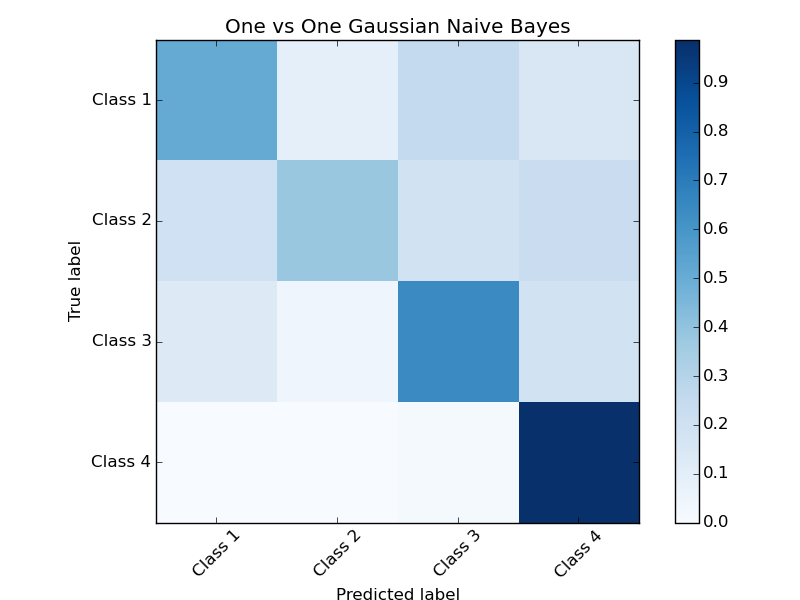
\includegraphics[width=\textwidth]{ovo_gnb.png}
		\caption{Gaussian Naive Bayes}
	\end{subfigure}
	%
	\begin{subfigure}[b]{0.5\textwidth}
		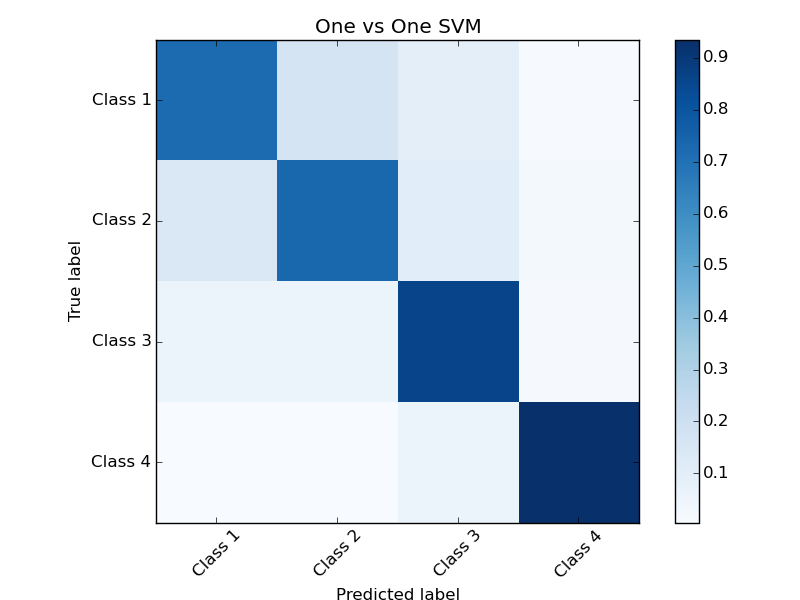
\includegraphics[width=\textwidth]{ovo_svm.png}
		\caption{Linear SVM}
	\end{subfigure}
	\caption{Confusion Matrix for One vs One Method}
	\label{fig:cm_ovo}
\end{figure}

\begin{figure}[h]
	
	\begin{subfigure}[b]{0.5\textwidth}
		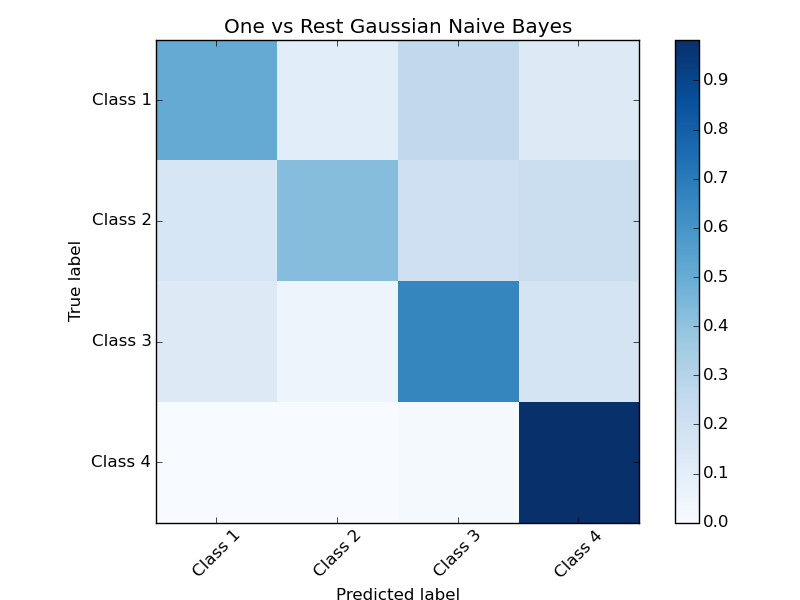
\includegraphics[width=\textwidth]{ovr_gnb.png}
		\caption{Gaussian Naive Bayes}
	\end{subfigure}
	%
	\begin{subfigure}[b]{0.5\textwidth}
		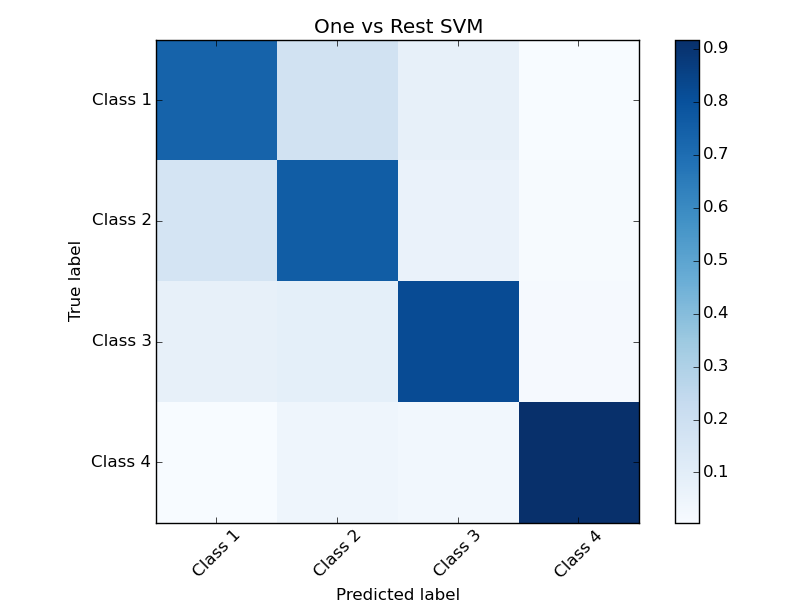
\includegraphics[width=\textwidth]{ovr_svm.png}
		\caption{Linear SVM}
	\end{subfigure}
	\caption{Confusion Matrix for One vs Rest Method}
	\label{fig:cm_ovr}
\end{figure}

\end{document}